\section{Situation}
	\paragraph{}
		Ce projet avait pour but de nous faire réaliser une architecture d'annuaire en installant des services qui reposent sur l'Active Directory et la supervision de serveurs. L'architecture a réaliser est pour le compte du groupe iSEC dont l'organisation est schématisé dans la figure \ref{isec_orga}.

		\begin{figure}[h]
			\centering
			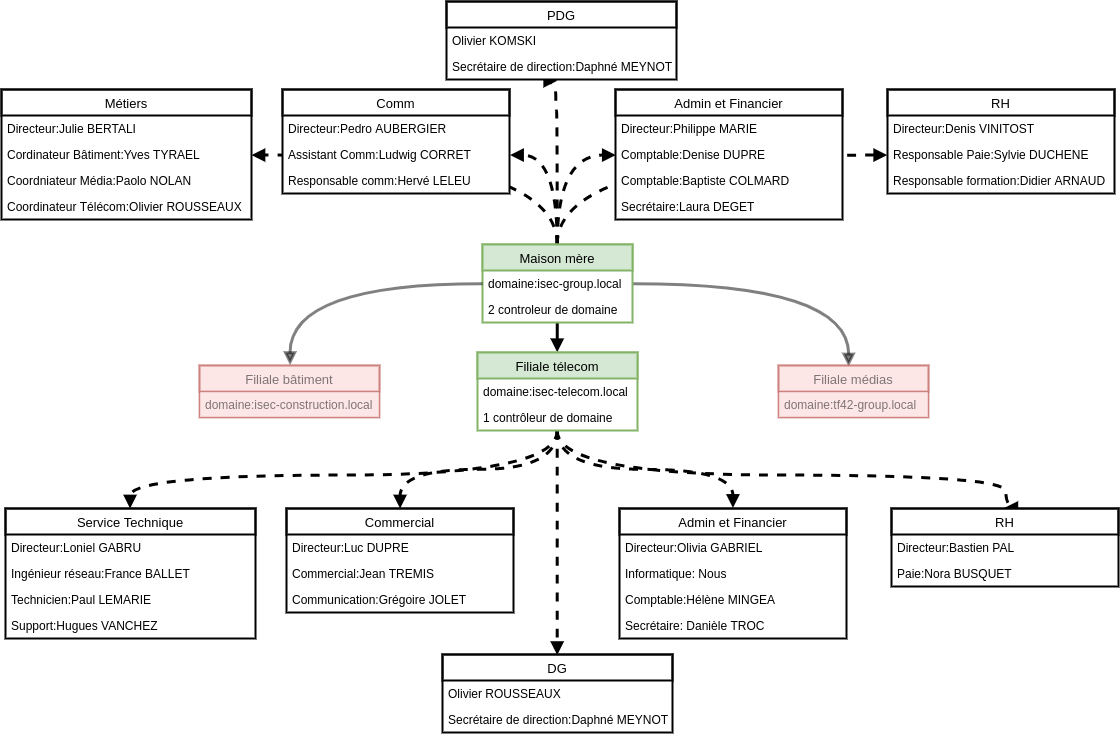
\includegraphics[scale=0.45]{Presentation/img/ISEC_orga.png}
			\caption{Schéma de l'organisation de groupe iSEC.}
			\label{isec_orga}
		\end{figure}
	\paragraph{}
		Le groupe iSEC, qui vient de racheter une entreprise, est présent dans plusieurs secteurs d'activités et possède donc plusieurs filiales. Il souhaite connecter le réseau de la maison mère avec celle des filiales. Notre but est de mettre en \oe{}uvre l'architecture Active Directory de la maison mère et de la filiale télécom uniquement.
	\subsection{Besoins techniques}
		\paragraph{}
			Les besoins techniques sont nombreux, mais le principal est de relier la maison mère et la filiale télécom avec un Active Directory. Le groupe iSEC doit avoir un contrôleur de domaine principal ainsi qu'un réplica pour la continuité de service. Le groupe télécom lui doit avoir un seul contrôleur de domaine. De plus une \textbf{relation d'approbation unidirectionnelle} entre les deux fôrets doit être mise en place, les utilisateurs du domaine groupe peuvent accéder aux ressources du domaine de la filiale télécom mais pas l'inverse.
		\paragraph{}	
			L'arborescence de l'Active Directory doit être créée et organisée selon les organigrammes du groupe et de sa filiale. De nombreux partages doivent ensuite être disponibles entre services, groupes et utilisateurs. D'autres service doivent être proposés par l'Active Directory comme l'installation automatique de 7Zip, la mise en place de fond d'écran et bien d'autre services qui sont décris dans les procédures d'installation qui suivent.
	\subsection{Organisation}
		\paragraph{}
			Ce projet a commencé le lundi 4 décembre et se termine le mardi 12 novembre. Les taches ont été découpées comme dans la figure \ref{planning} :

			\begin{figure}[h]
				\centering
				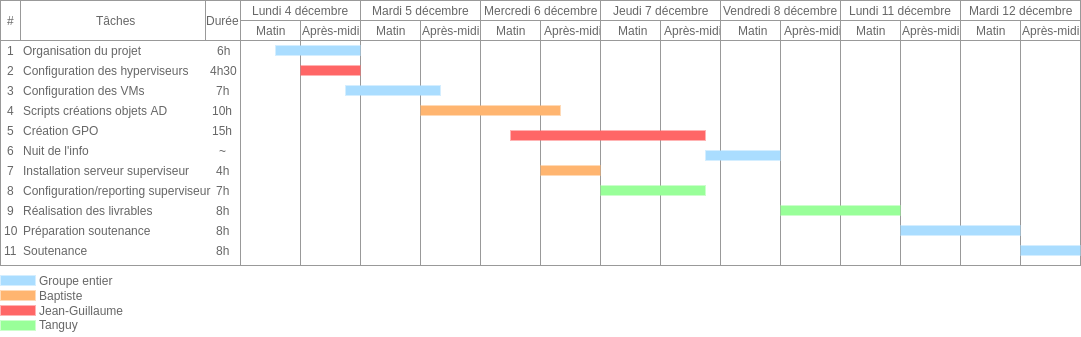
\includegraphics[scale=0.50]{Presentation/img/Planning_previsio.png}
				\caption{Planning prévisionnel du projet.}
				\label{planning}
			\end{figure} 

		\paragraph{}
			Ce planning prévisionnel a été dans l'ensemble respecté, certaines heures supplémentaires ont été nécessaires pour la configuration des serveurs de supervision. Un dépot Github a été créé afin de conserver les différents scripts utilisés pendant ce projet ainsi que les sources de ce rapport, il est disponible à ce lien : \href{https://github.com/Exia-epickiwi/Projet-iSEC}{https://github.com/Exia-epickiwi/Projet-iSEC}